\section{Algoritmo parallelo}

La popolazione di cellule è modellata tramite un array, una delle strutture
dati più adatte ad essere parallelizzate su GPU, dato che è possibile
demandare la computazione di ogni elemento dell'array ad uno specifico thread.
Sia la creazione che la simulazione della proliferazione fanno uso solamente di
array unidimensionali, dunque il problema rimane solamente la stesura di un
algoritmo in grado di massimizzare il parallelismo per computazione
dell'insieme di array necessario a portare a termine la simulazione. 

% Descrizione della creazione della popolazione iniziale partendo dal file
% dell'istogramma di partenza
\subsection{Creazione della popolazione iniziale}

L'istogramma $H(0)$ che riporta i valori di fluorescenza con la rispettiva
frequenza è salvato su un file di testo che deve essere letto in modo
sequenziale. Una volta letto l'intero file avremo creato un array i cui
elementi saranno le coppie di valori $(\varphi_{i}, \psi_{i})$.
Ora che è nota la frequenza $\psi_{i}$ per ogni fluorescenza $\varphi_{i}$,
è possibile invocare l'esecuzione di un \textit{kernel} per ogni coppia di
valori tale che al kernel vengano assegnati esattamente $\psi_{i}$ thread,
in modo tale che ognuno di essi si occupi di generare una cellula avente $\varphi_{i}$
valore di fluorescenza.
\\
\begin{figure}[H]
    \centering
    \begin{tikzpicture}
        \pgftransparencygroup
        \nodes{(\varphi_{i}, \psi_{i})}
        \endpgftransparencygroup
        \pgftransparencygroup
        \hiddennodes{$\longrightarrow$}
        \endpgftransparencygroup
        \pgftransparencygroup
        \nodes{\varphi_{i}, \varphi_{i}}
        \endpgftransparencygroup
        \pgftransparencygroup
        \hiddennodes{., ., .}
        \endpgftransparencygroup
        \pgftransparencygroup
        \nodes{\varphi_{i}, \varphi_{i}}
        \endpgftransparencygroup
    \end{tikzpicture}
    \caption{}
\end{figure}

% Descrizione dell'avanzamento della simulazione
\subsection{Simulazione della proliferazione cellulare}

L'idea generale è che dato l'array della popolazione iniziale $X_{0}$
sia possibile per ogni elemento $X_{0,i}$ in esso contenuto sviluppare
la simulazione creando due nuove cellule figlie partendo da una cellula
originaria, ovvero l'elemento selezionato dall'array iniziale.
\\
Per la simulazione viene invocato un \textit{kernel} specifico.
Sia $X_{0,i}$ un elemento dell'array iniziale
con $i < L$, a cui è associato un certo valore $\varphi_{j}$
con $j < |\varphi|$ e sia $X_{1}$ un array rappresentante la nuova
popolazione cellulare.
Dal \textit{kernel} invocato, per ogni $X_{0,i}$ viene dedicato un GPU thread,
che svolgerà le seguenti procedure.
\\
Le nuove cellule generate dalla proliferazione
di $X_{0, i}$ saranno $$X_{1, (2 * i)}$$ $$X_{1, (2 * i + 1)}$$

Esse avranno il proprio tempo di vita globale $\tau$
incrementato secondo la seguente
$$\tau[X_{1, (2 * i)}] = \tau[X_{0, i}] + \mu[X_{0, i}]$$
dove $\mu[X_{0, i}]$ indica il tempo dopo il quale la cellula $X_{0,i}$
procede alla propria divisione.
\\
La simulazione prevede un tempo massimo $\tau_{max}$ e una soglia minima
$\varphi_{min}$ entro il quale procedere
alla divisione di una cellula, dunque il fenomeno appena descritto avviene
solamente se $\tau[X_{0, i}] + \mu[X_{0, i}] \leqslant \tau_{max}$ oppure se
$\varphi[X_{0, i}] / 2 \geqslant \varphi_{min}$.
Questa restrizione implica che all'interno di $X_{1}$ alcuni elementi non
vengano computati. Per ovviare a questo inconveniente è stato deciso di
assegnare ad ogni cellula uno stato locale $\{Alive, Inactive, Remove\}$
indicatore del fatto che la cellula
può oppure non può più procedere ulteriormente con la divisione.
\\
Sia $\sigma$ l'array degli stati di ogni cellula, allora possiamo riassumere
l'assegnazione degli stati come segue
$$\tau[X_{1, (2 * i)}] = \tau[X_{0, i}] + \mu[X_{0, i}] \leqslant \tau_{max}
\longrightarrow \sigma[X_{1, (2 * i)}] = \sigma[X_{1, (2 * i + 1)}] = Alive$$
$$\tau[X_{1, (2 * i)}] = \tau[X_{0, i}] + \mu[X_{0, i}] \geqslant \tau_{max}
\longrightarrow \sigma[X_{1, (2 * i)}] = Inactive \land
\sigma[X_{1, (2 * i + 1)}] = Remove$$
$$\varphi[X_{1, (2 * i)}] = \varphi[X_{0, i}] / 2 \leqslant \varphi_{min}
\longrightarrow \sigma[X_{1, (2 * i)}] = \sigma[X_{1, (2 * i + 1)}] = Remove$$

Una volta che il kernel ha terminato l'esecuzione di tutti i thread, il
controllo viene ritornato alla CPU.
Gli stati risultano necessari poichè dopo l'evento di proliferazione cellulare
dobbiamo procedere all'aggiornamento dei risultati rimuovendo
da $X_{1}$ le cellule $Inactive$ e aggiungendole ad un nuovo array dei
risultati $P$.
Procediamo inoltre all'eliminazione delle cellule con stato $Remove$ in quanto
possiedono un valore di fluorescenza $\varphi$ sotto la soglia $\varphi_{min}$.
L'array risultante conterrà solamente cellule $Alive$, dunque possiamo
utilizzare $X_{1}$ come nuovo array iniziale e reiterare
il processo appena descritto fino a quando non saranno più presenti cellule
$Alive$.
Terminate le iterazioni l'array $P$ conterrà tutte e sole le cellule che hanno
superato il limite temporale $\tau_{max}$, dunque è possibile calcolare
l'istogramma dei risultati utilizzando la funzioni definite dalle librerie
\textit{Thrust}\cite{bell2011thrust} di CUDA e salvare il risultato ottenuto
su file.

\begin{figure}[H]
    \centering
    \begin{tikzpicture}
        \begin{axis}[legend pos=outer north east,
                xtick=data,
                xlabel={$\tau_{max}$},
                ylabel={simulation time (s)}
            ]
            \addplot table[x=Time, y=Python] {Data/Accelerants/fit.txt};
            \addplot table[x=Time, y=Original] {Data/Accelerants/fit.txt};
            \legend{Python,CUDA}
        \end{axis}
    \end{tikzpicture}
    \caption{}
\end{figure}

Come è possibile notare dal grafico, è presente un aumento delle performance
rispetto alla versione procedurale dell'algoritmo, ma non è ancora degno
di nota per quanto riguarda i risultati che si vogliono ottenere.

% Spiegazione dei metodi per accelerare la computazione
\subsection{Acceleranti}

Sebbene la soluzione descritta in precedenza sia corretta, come mostrato nei
grafici è evidente che bisogna cercare di migliorare ulteriormente
l'algoritmo in modo da renderlo ancora più performante, in quanto uno
speedup di \textbf{8x} non è sufficiente per preferire questa soluzione
rispetto ad una procedurale considerando anche il fattore costo per le moderne
GPU rispetto alle CPU in commercio.
È anche da tenere in considerazione il fatto che l'algoritmo si appoggia
ancora molto sulla CPU quando si tratta di iterare l'array delle soluzioni.
Detto questo è necessario implementare alcuni \textit{acceleranti} per
incrementare le perfomance e rendere questa soluzione preferibile rispetto
all'algoritmo scritto per la CPU.

% Descrizione del parallelismo dinamico
\paragraph{Parallelismo dinamico}

NVIDIA dalla versione \textit{5.0} di CUDA e su architetture hardware a partire
dalla versione \textit{compute\_35} ha introdotto la possibilità di invocare
l'esecuzione di un kernel da un altro kernel.
Questa pratica è viene definita
\textit{Parallelismo Dinamico}\cite{jones2012introduction} in quanto permette
di computare strutture intrinsecamente ricorsive, dato che da un kernel può
essere invocato lo stesso kernel con parametri differenti come ad 
esempio l'implementazione del \textit{radix sort}\cite{merrill2011high}.
\\
L'idea è utilizzare il parallelismo dinamico per computare non solo il primo
livello degli alberi di proliferazione cellulare, ma proseguire fino ad arrivare
all'ultimo livello, ritornando il controllo alla CPU solo in questo caso.
Per effettuare questa operazione bisogna sfruttare al massimo il concetto di
\textit{Thread Block} dato che CUDA offre la possibilità di sincronizzare
tutti i thread appartenenti ad un blocco tramite la primitiva
\textit{\_\_syncthreads()}\cite{jones2012introduction}.
L'array $X_{1}$ viene computato da $\ceil*{L/2^{10}}$ \textit{Thread Block},
invece di terminare la computazione è possibile continuare a computare
gli array successivi $X_{2}...X_{n}$ a blocchi, ovvero sincronizzare i thread
all'interno di un \textit{Thread Block} tramite la primitiva
\textit{\_\_syncthreads()} e in seguito invocare l'esecuzione di un nuovo kernel
utilizzando però $2$ \textit{Thread Block} dato che il blocco corrente ha
generato $2 * 2^{10}$ cellule appartenenti al livello successivo dell'albero.
\\
\begin{figure}[H]
    \begin{minipage}[b]{.5\linewidth}
    \centering
    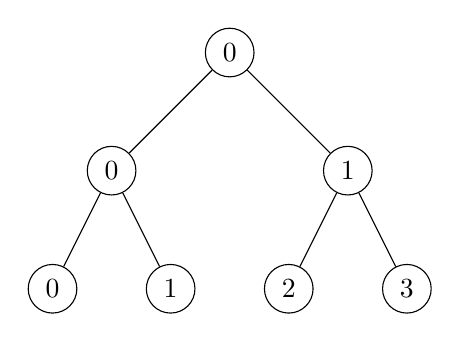
\begin{tikzpicture}[level/.style={sibling distance=30mm/#1}]
        \node [circle, draw] (a) {$0$}
            child {
                node [circle,draw] (b) {$0$}
                    child {
                        node [circle,draw] (d) {$0$}
                    }
                    child {
                        node [circle,draw] (e) {$1$}
                    }
            }
            child {
                node [circle,draw] (c) {$1$}
                    child {
                        node [circle,draw] (f) {$2$}
                    }
                    child {
                        node [circle,draw] (g) {$3$}
                    }
            };
    \end{tikzpicture}
    \end{minipage}
    \begin{minipage}[b]{.5\linewidth}
    \centering
    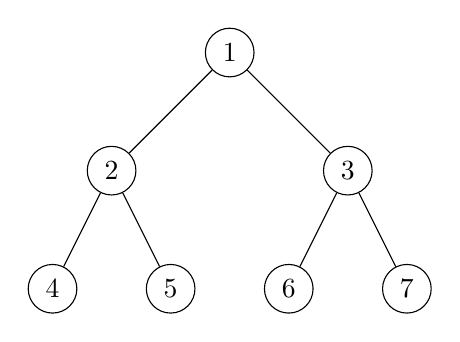
\begin{tikzpicture}[level/.style={sibling distance=30mm/#1}]
        \node [circle, draw] (a) {$1$}
            child {
                node [circle,draw] (b) {$2$}
                    child {
                        node [circle,draw] (d) {$4$}
                    }
                    child {
                        node [circle,draw] (e) {$5$}
                    }
            }
            child {
                node [circle,draw] (c) {$3$}
                    child {
                        node [circle,draw] (f) {$6$}
                    }
                    child {
                        node [circle,draw] (g) {$7$}
                    }
            };
    \end{tikzpicture}
    \end{minipage}
    \caption{}
\end{figure}

In figura possiamo vedere due alberi di proliferazione, dove ogni nodo
rappresenta l'indice di una cellula all'interno dell'array della popolazione
corrispondente al livello degli alberi considerato, come segue:

\begin{itemize}
    \item $X_{0} = [0, 1]$
    \item $X_{1} = [0, 1, 2, 3]$
    \item $X_{2} = [0, 1, 2, 3, 4, 5, 6, 7]$    
\end{itemize}

Denotiamo con $B_{i,j}$ un generico \textit{Thread Block} dove
$i$ rappresenta la popolazione $X_{i}$, mentre $j$ l'indice del blocco.
Quindi $B_{0,0} = [0, 1]$ sarà il blocco che date le
cellule $[0, 1] \subseteq X_{0}$ si occupa di
computare le figlie risultanti dalla divisione, ovvero
$[0, 1, 2, 3] \subseteq X_{1}$.
Al termine della computazione di $B_{0,0}$, viene invocata la primitiva 
\textit{\_\_syncthreads()} ed eseguito un nuovo kernel, che istanzierà
i blocchi $B_{1,0} = [0, 1]$ e $B_{1,1} = [2, 3]$, che a loro volta
eseguiranno $B_{2,0} = [0, 1]$, $B_{2,1} = [2, 3]$,
$B_{2,2} = [4, 5]$ e $B_{2,3} = [6, 7]$.
\\
Questo metodo accelera di molto l'esecuzione dell'algoritmo, ma introduce un
ulteriore problema: a priori non è possibile conoscere la profondità esatta
degli alberi di proliferazione, dato che si tratta di una simulazione
di tipo stocastico, dunque l'utilizzo di memoria aumenta esponenzialmente
all'aumentare dei livelli di profondità degli alberi.
\\
Un altro problema che è sorto è la limitazione hardware del parallelismo
dinamico, ovvero il fatto che è possibile innestare solamente un massimo
di \textbf{24 livelli} di ricorsione. Questo fatto ci costringe a dover
eventualmente terminare la ricorsione e ritornare il controllo alla CPU,
iterando nuovamente fino a raggiungere il termine della simulazione.

\begin{figure}[H]
    \centering
    \begin{tikzpicture}
        \begin{axis}[legend pos=outer north east,
                xtick=data,
                xlabel={$\tau_{max}$},
                ylabel={simulation time (s)}
            ]
            \addplot table[x=Time, y=Original] {Data/Accelerants/fit.txt};
            \addplot table[x=Time, y=Dynamic] {Data/Accelerants/fit.txt};
            \legend{CUDA, Dynamic parallelism}
        \end{axis}
    \end{tikzpicture}
    \caption{}
\end{figure}

Dal grafico in figura è possibile vedere l'aumento significativo delle
performance rispetto alla versione che non presenta l'utilizzo del
parallelismo dinamico. Questo è dovuto al fatto che la sincronizzazione
di tutti i blocchi delle GPU che deve essere effettuata al termine di ogni
iterazione è molto onerosa in termini prestazionali, inoltre anche la copia
dei dati da GPU a CPU per l'aggiornamento dell'array dei risultati risulta
particolarmente time-consuming.

% Descrizione del metodo di bound
\paragraph{Bounding}

Sebbene il parallelismo dinamico introduca un enorme vantaggio, porta con sè
una limitazione importante, ovvero il fatto che un kernel non termina la sua
esecuzione fino a quando tutti i kernel invocati da quest'ultimo non sono
anch'essi terminati. Durante la computazione degli alberi questo può portare
ad alcuni rallentamenti, dato che è inutile computare rami le cui cellule
sono state marcate come $Inactive$ o $Remove$ dato che non contribuiscono
alla creazione del nuovo livello di proliferazione.
Detto questo risulta utile tenere traccia del fatto che un \textit{Thread Block}
abbia oppure no generato nuove cellule.
In questo caso ci viene in aiuto la \textit{Shared Memory}\cite{sanders2010cuda}
, ovvero una zona di memoria condivisa tra tutti i thread appartenenti ad
uno stesso \textit{Thread Block}. Utilizzando quest'area di memoria è possibile
settare un flag indicante il fatto che è avvenuto un evento di proliferazione
cellulare. Se ci trovassimo nel caso in cui nessun evento è avvenuto, sarebbe
inutile invocare un nuovo kernel, quindi la computazione dei successivi
sotto-alberi viene interrotta.
\\
Siano $A = Alive$, $I = Inactive$, $R = Remove$, il metodo implementato
produce i seguenti risultati

\begin{figure}[H]
\begin{minipage}[b]{.5\linewidth}
\centering
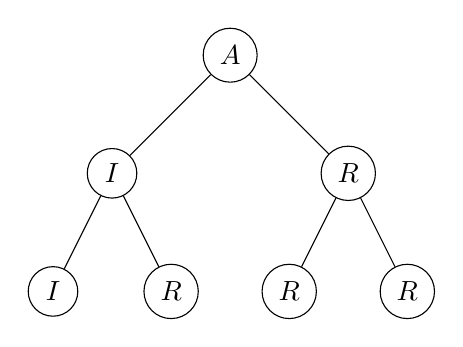
\begin{tikzpicture}[level/.style={sibling distance=30mm/#1}]
    \node [circle, draw] (a) {$A$}
        child {
            node [circle,draw] (b) {$I$}
                child {
                    node [circle,draw] (d) {$I$}
                }
                child {
                    node [circle,draw] (e) {$R$}
                }
        }
        child {
            node [circle,draw] (c) {$R$}
                child {
                    node [circle,draw] (f) {$R$}
                }
                child {
                    node [circle,draw] (g) {$R$}
                }
        };
\end{tikzpicture}
\subcaption{Senza bounding}
\end{minipage}
\begin{minipage}[b]{.5\linewidth}
\centering
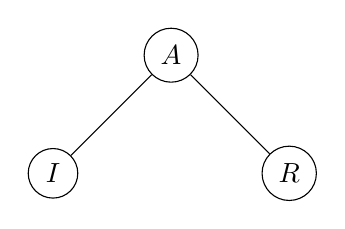
\begin{tikzpicture}[level/.style={sibling distance=30mm/#1}]
    \node [circle, draw] (a) {$A$}
        child {
            node [circle,draw] (b) {$I$}
        }
        child {
            node [circle,draw] (c) {$R$}
        };
\end{tikzpicture}
\subcaption{Bounding}
\end{minipage}
\caption{}
\end{figure}

\begin{figure}[H]
    \centering
    \begin{tikzpicture}
        \begin{axis}[legend pos=outer north east,
                xtick=data,
                xlabel={$\tau_{max}$},
                ylabel={simulation time (s)}
            ]
            \addplot table[x=Time, y=Dynamic] {Data/Accelerants/fit.txt};
            \addplot table[x=Time, y=Bounding] {Data/Accelerants/fit.txt};
            \legend{Dynamic parallelism, Bounding}
        \end{axis}
    \end{tikzpicture}
    \caption{}
\end{figure}

Il leggero aumento delle prestazioni mostrato in figura indica che la tecnica
del \textit{bounding} ha poco impatto sull'aumento delle performance, ma
sicuramente contribuisce alla migliore gestione delle risorse computazionali
relative alla GPU e all'uso intensivo del parallelismo dinamico.

% Descrizione del metodo di inferenza della profondità dell'albero
\paragraph{Inferenza del livello di profondità}

Sebbene CUDA ci ponga un livello massimo di nesting pari a $24$ livelli,
nei modelli presi in considerazione per queste simulazioni, difficilmente
si supera la soglia dei $5$ eventi di proliferazione per ogni cellula,
però per come è stato pensato l'utilizzo del parallelismo dinamico vengono
allocati $N$ livelli pari al numero massimo di cellule che è possibile mantenere
sulla memoria della GPU, dunque se in memoria centrale è presente sufficiente
spazio per allocare $10$ livelli di profondità essi vengono allocati,
consumando più risorse del necessario. Non è nemmeno possibile utilizzare
la memoria di \textit{swap} dato che le schede non supportano questa
funzionalità.
È necessario quindi trovare un modo per inferire nel modo più accurato
possibile il numero di livelli necessari alla simulazione.
Un modo banale è quello di dare la possibilità all'utente di specificare il
numero di livelli da utilizzare durante la simulazione, se è al corrente
del numero media di divisioni che ogni cellula andrà ad affrontare.
Un altro modo è quello di inferire il livello utilizzando i parametri forniti
in ingresso alla simulazione.
Per poter calcolare i diversi tipi di cellule, si utilizza un array di
parametri contenente le distribuzioni uniformi $\pi$ dei vari tipi di cellule
$\tau$ che è possibile avere all'interno della popolazione iniziale.
Ogni tipo di cellula possiede un tempo medio $\mu$ dopo il quale avviene
la divisione, il quale segue una distribuzione normale.
È possibile pensare di utilizzare il tempo medio $\mu_{i}$ del tipo di cellula
$\tau_{i}$ che ha probabilità $\pi_{i}$ maggiore per calcolare un numero
approssimativo di livello di divisioni tali per cui venga superato il
$\tau_{max}$ definito per la simulazione.
\\
Sia $\mu_{max}$ il tempo medio di divisione
del tipo di cellula avente $max(\pi)$.
Allora possiamo stimare che il numero $\eta$ dei livelli di profondità
dell'albero è $$\eta : \sum\limits_{i=1}^{\eta - 1}
\mu_{max} \leqslant \tau_{max} \leqslant \sum\limits_{i=1}^{\eta} \mu_{max}$$

\begin{figure}[H]
    \centering
    \begin{tikzpicture}
        \begin{axis}[legend pos=outer north east,
                xtick=data,
                xlabel={$\tau_{max}$},
                ylabel={simulation time (s)}
            ]
            \addplot table[x=Time, y=Bounding] {Data/Accelerants/fit.txt};
            \addplot table[x=Time, y=Inference] {Data/Accelerants/fit.txt};
            \legend{Bounding, Inference}
        \end{axis}
    \end{tikzpicture}
    \caption{}
\end{figure}

% Descrizione della costruzione dell'istogramma finale
\paragraph{Calcolo dell'istogramma finale}

Sebbene le performance siano aumentate, il software fa ancora molto affidamento
sulla CPU per il calcolo dell'istogramma finale.
Ad ogni iterazione l'array della popolazione $X_{n}$ viene trasferito
attraverso la CPU in memoria centrale per essere filtrato e per aggiornare i
risultati dell'istogramma. Questo processo è possibile grazie alla funzione
\textit{cudaMemcpy()} che si occupa del trasferimento dei dati tra CPU e GPU.
Diverse chiamate a questa funzione generano un lavoro intensivo che deve essere
effettuato, quindi impatta ulteriormente sullo speedup della simulazione.
L'obiettivo è quindi cercare di minimizzare il numero di trasferimenti tramite
\textit{cudaMemcpy()}.
\\
La soluzione risiede nella possibilità di calcolare l'istogramma direttamente
sulla GPU. Assumendo di conoscere un array ordinato in modo crescente$\Omega$
contenente tutti possibili valori di fluorescenza
$\varphi$ che una cellula potrà assumere in futuro, è possibile far eseguire
ad un thread del kernel (se computando una cellula $Active$ essa non è più in
grado di proliferare) una ricerca binaria su $\Omega$ e aggiornare
il valore di frequenza $\psi$ corrispondente alla fluorescenza trovata, tramite
la funzione $atomicAdd()$ di CUDA, la quale anche se prevede una
sincronizzazione sulla risorsa a cui si vuole accedere, è necessaria dato che
ad ora non esiste un altro modo per il calcolo di un istogramma attraverso un
algoritmo parallelo.
\\
Conoscendo l'istogramma iniziale $H(0)$ in realtà abbiamo già a disposizione
tutti i valori di fluorescenza che una cellula potrà assumere, infatti
$\Omega$ conterrà tutti i valori di $H(0)$ tali che $\varphi_{i} \geqslant
\varphi_{min}$ e i successivi valori $\varphi_{i}^{-2j}$ con $j \in \N, j > 0$.
\\
Questa tecnica evita il trasferimento dati al termine di ogni iterazione, poichè
la frequenza riguardante i valori di fluorescenza delle cellule $Inactive$
è già stata aggiornata durante l'esecuzione del kernel.
Mediante questa tecnica la $cudaMemcpy()$ viene utilizzata solamente a inizio
e fine simulazione per il salvataggio dei risultati.

\begin{figure}[H]
    \centering
    \begin{tikzpicture}
        \begin{axis}[legend pos=outer north east,
                xtick=data,
                xlabel={$\tau_{max}$},
                ylabel={simulation time (s)}
            ]
            \addplot table[x=Time, y=Inference] {Data/Accelerants/fit.txt};
            \addplot table[x=Time, y=Histogram] {Data/Accelerants/fit.txt};
            \legend{Inference, Histogram}
        \end{axis}
    \end{tikzpicture}
    \caption{}
\end{figure}

Come si evince dai grafici, questo è l'accelerante che incrementa maggiormente
lo speedup dell'algoritmo, dato che risolve quasi totalmente il problema
del bottleneck causato dal trasferimento bidirezionale delle informazioni
per lo svolgimento della simulazione.

% Descrizione del problema della gestione della memoria
\subsection{Gestione della memoria}

L'implementazione degli acceleranti ha migliorato di gran lunga le
performance dell'algoritmo, ma ha introdotto un problema, ovvero la crescita
esponenziale della memoria.
Infatti data la numerosità $L$ della popolazione iniziale $X_{0}$, essa cresce
esponenzialmente con il numero dei livelli dell'albero $L * 2^i$ con
$i \in \N, i > 0$. Inizialmente questa crescita era mitigata dal fatto che
dopo ogni iterazione la popolazione veniva filtrata, quindi procedendo verso
il termine della simulazione, l'utilizzo di memoria veniva bilanciato dalla
poca numerosità delle cellule $Alive$ rimanenti.
Dopo l'introduzione dell'ultimo accelerante, sebbene le cellule $Inactive$ e
$Remove$ non vengano prese in considerazione per la computazione, sono
comunque presenti ancora all'interno delle diverse popolazioni, dato che
dopo ogni iterazione la memoria non viene più filtrata in quanto non più
trasferita sulla CPU.

\begin{figure}[H]
    \centering
    \begin{tikzpicture}
        \begin{axis}[legend pos=north west,
                xtick=data,
                xlabel={iterations},
                ylabel={final population size (MB)}
            ]
            \addplot table[x=Iteration, y=Serial] {Data/Memory/validation.txt};
            \addplot table[x=Iteration, y=Parallel] {Data/Memory/validation.txt};
            \legend{Serial histogram,Parallel histogram}
        \end{axis}
    \end{tikzpicture}
    \caption{}
\end{figure}

La crescita esponenziale dell'occupazione di memoria potrebbe essere un
problema nel momento in cui il tempo $\tau_{max}$ inizia a crescere
ulteriormente. La soluzione immediata a questo problema potrebbe essere di
natura economica, ovvero l'acquisto di GPU moderne con molta memoria a
disposizione. Il problema però persiste, quindi una possibile soluzione
potrebbe essere quella di computare ad un certo punto solamente un sottoinsieme
della popolazione e trasferire i restanti elementi sulla CPU, per poi
elaborarli nuovamente quando il primo sottoinsieme di popolazione è stato
elaborato. Questo però introdurrebbe nuovamente la necessità di utilizzare
in modo assiduo $cudaMemcpy()$, però fino ad ora pare essere l'unica soluzione
plausibile.
